\documentclass[a4paper, 10pt, conference]{IEEEtran}
\usepackage{enumitem}
\usepackage{graphicx,float}
\usepackage{subcaption}

\newcommand{\head}[1]{\textnormal{\textbf{#1}}}

\title{Predicting the Outcome of ODI Cricket Matches using Decision Trees and MLP Networks}

\author{
\IEEEauthorblockN{Rajiv Kumar\IEEEauthorrefmark{1},Jalaz Kumar\IEEEauthorrefmark{2}}
\IEEEauthorblockA{
\IEEEauthorrefmark{1}Assistant Professor,\IEEEauthorrefmark{2}Student\\
Department of Computer Science and Engineering\\
National Institute of Technology Hamirpur, India\\
Email: \IEEEauthorrefmark{1}rajiv@nith.ac.in,\IEEEauthorrefmark{2}jalazkumar1208@gmail.com}}

\begin{document}

\maketitle
\thispagestyle{empty}
\pagestyle{empty}


%%%%%%%%%%%%%%%%%%%%%%%%%%%%%%%%%%%%%%%%%%%%%%%%%%%%%%%%%%%%%%%%%%%%%%%%%%%%%%%%
\begin{abstract}

Applying Data Mining \& Machine Learning in Sports Analytics is a blooming sector in the field of Computer Science. After Football, Cricket is the second most popular sports with a fan base of around 2.5 billion and mostly popular in South Asia, Australia, The Caribbeans and UK. It has tremendous spectator support and the masses show great interest in predicting the outcome of games.
The result of a cricket match depends on lots of in-game and pre-game attributes. Pre-game attributes like venue,past track-records, Innings(First/Second), team strength etc. and in-game attributes like Toss, run rate, wickets in hand, strike rate etc. influence a match result predominantly. 
In our study, we have used 2 different ML approaches, Decision Trees \& MultiLayer Perceptron Network, to predict how these factors affect the outcome of an ODI cricket match. Based on the emerged results, We have designed CricAI: Cricket Match Outcome Prediction System. Our designed tool takes into consideration the pre-game attributes like ground,  venue(home,away,neutral) \& innings(first/second) to predict the outcome of given match.


Keywords: Decision Tree Classifier, MLP Classifier, Features, Performance Measures

\end{abstract}


%%%%%%%%%%%%%%%%%%%%%%%%%%%%%%%%%%%%%%%%%%%%%%%%%%%%%%%%%%%%%%%%%%%%%%%%%%%%%%%%
\section{INTRODUCTION}

Cricket which is the world's second most popular sport after soccer, is basically a bat and ball game played between two teams of eleven players each. Each teams comes to bat and has a single inning in which it seeks to score as many runs as possible, while the other team fields. The innings ends when the total quota of deliveries, which depends on game format have turned up, or the 10 batsman has been dismissed, whichever comes first. The prime objective is to score more runs \& thus Runs are the decisive factor.

Game of Cricket is highly unpredictable in nature. Till the very last moment, it is difficult to make accurate predictions about the game. Various natural factors affecting the game output, huge betting market and enormous media coverage have given strong incentives to model this gentlemans' game from the Machine Learning perspective.

Rules of Cricket are determined by the International Cricket Council(ICC).

There are three internationally recognized formats of Cricket matches - Test match, ODI match(One Day International) and T20 match. The main difference between these three formats is the scheduled duration of the game which directly modifies the number of deliveries each team got to play in their respective innings.

Test cricket format is the longest one and is considered as the highest standard of game. Match duration is five days in which each team get to play 2 innings each. A standard test cricket day consist of 3 sessions of 2 hours each.

One Day International i.e. ODI format is of limited overs, where each team faces 300 deliveries(50 overs). ODI match is scheduled to complete in a Day or a Day/Night combination.

T20 is the shortest internationally recognized format of this game, where each team innings consist of 20 overs. This is more of an "explosive" and more "athletic" than the other two formats.

We focus our research on One Day Internationals, the most popular format of the game. Outcome of ODI match is influenced by a large no. of factors and  can be predicted like all other games. We need to find the best attributes or factors that influence the match outcome. For our study we considered the factors analyzed by [1] and [2], which are proven to have a significant impact on outcome of ODI match. The factors considered for analysis include:

\begin{description}
  \item[$\bullet$ Teams Past Performance:] This factor captures the historic outcomes of all the matches played between the teams.
  \item[$\bullet$ Ground:] This plays a vital role as teams have great track records on grounds and carry psychological superiority over the other.
  \item[$\bullet$ Innings:] This factor determines which team batted first \& which batted second.
  \item[$\bullet$ Home Game Advantage:] This is achieved by using Venue feature, which determines whether a particular ground is home/away/neutral for each of the playing teams.
\end{description}

Both of our classifiers are trained on the basis of these factors. For predicting the outcome of ODI matches we have used 2 supervised classification techniques - Decision Trees and Multi-Layer Perceptron Networks. We have conducted comparative studies between both the classifiers and summarized the results in this paper.

We then built a software tool called CricAI based on emerged results, which can be used to predict the outcome of any ODI match given the concerned factors as inputs. This software of ours can be of real value to the cricketers, support staff of teams and cricket analysts in terms of analyzing the future game in advance and working towards maximizing their chances of victory.

Clustering couldn't have made any contribution to our research as we dealt with multiple independent attributes, therefore placing them in clusters after finding similarity did not seem feasible.

The rest of this paper is organised as follows. Section 2 explains the approach we have used for conducting the analysis. Section 3 presents a comparative study of the classifiers used. Section 4 presents the related work in the area. Section 5 gives the conclusions and the future scope associated with this approach.\\

%%%%%%%%%%%%%%%%%%%%%%%%%%%%%%%%%%%%%%%%%%%%%%%%%%%%%%%%%%%%%%%%%%%%%%%%%%%%%%%%%%%%%
\section{APPROACH FOR ANALYSIS}

\subsection{Data Collection}

Data was extracted from [1] by running a scraping script in a justified manner, sending 1 request per second.
\begin{table}[h!]
  \begin{center}
    \caption{Scrapped Dataset Format}
    \label{tab:table1}
    \begin{tabular}{cccccc} 
      \textbf{Match Id} & \textbf{Team 1} & \textbf{Team 2} & \textbf{Winner} & \textbf{Margin} & \textbf{Ground}\\
      \hline
      ODI \#1 & Australia & England & Australia & 5 wickets & Melbourne\\
      ODI \#2 & England & Australia & England & 6 wickets & Manchester\\
      ODI \#3 & England & Australia & Australia & 5 wickets & Lord's\\
    \end{tabular}
  \end{center}
\end{table}

Dataset comprises of all the ODI matches from Jan 5, 1971 to Oct 29, 2017. A total of 3933 ODIs match results were scrapped. The collected data was subjected to cleaning process where some of the matches were deleted from the analysis. Since the impact of the nature on the game of cricket cannot be foreseen, matches which were either interrupted by rain or ended up in a draw/tie, were being removed from the dataset. Matches of Special teams like World XI, Asia XI \& Africa XI were also removed.

We also further replicated our dataset two times by swapping the team positions i.e. A game between Team 1: India and Team 2: Sri Lanka was also replicated as Team 1: Sri Lanka and Team 2: India.
For further making the dataset suitable for input to the various Machine Learning Classifier Models, we converted the continous dataset into a categorial dataset, using dummy variables.

\textbf{Innings Feature} was determined by first translating Column: \textit{Margin} into Column: \textit{Winner Innings} using:\\
\indent \indent $\cdot$ Win by Wickets  $\Longrightarrow$  Winner Innings: 2\\
\indent \indent $\cdot$ Win by Runs \indent $ \Longrightarrow$  Winner Innings: 1
\\Further, Using Column: \textit{Winner} and the generated  Column: \textit{Winner Innings}, we aquired the innings of each team per match.

\textbf{Venue Feature} was determined by using Column: \textit{Winner} and Scrapped dataframe from [1] which provided the names of cricket grounds in all countries. Combining both of these, Column: \textit{Host Country} was generated, which was used to get venue of a match with respect to both the teams.

The data set was saved in comma separated format. A total of 7494 match records were used in analysis.  Finally, we divided the dataset into two parts, namely, the test data and the training data.
\\$\star$ Training Dataset Size: 5620
\\$\star$ Testing Dataset Size: 1874

\subsection{MultiLayer Perceptron Networks}
Multi-layer Perceptron (MLP) is a supervised learning algorithm that learns a function \[ f(.): R^{m} \rightarrow R^{o} \] by training on a dataset, where \textit{m} is the number of dimensions for input and \textit{o} is the number of dimensions for output. Given a set of features \textit{X = $x_{1}$, $x_{2}$, ..., $x_{m}$} and a target \textit{y}, it can learn a non-linear function approximator for either classification or regression. It is different from logistic regression, in that between the input and the output layer, there can be one or more non-linear layers, called hidden layers. Fig 1. shows a Perceptron Network with 1 hidden layer.
\begin{figure}
  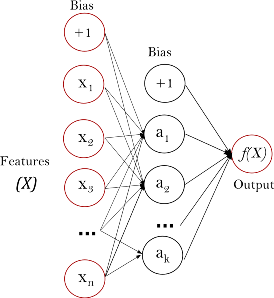
\includegraphics[width=\linewidth]{MLP.png}
  \caption{Multilayer Perceptron Network}
  \label{fig:mlp}
\end{figure}

The leftmost layer, known as the input layer, consists of a set of neurons \[ {x_{i}|x_{1},x_{2},\ldots,x_{m}} \] representing the input features. Each neuron in the hidden layer transforms the values from the previous layer with a weighted linear summation, \[ w_{1}x_{1} + w_{2}x_{2} + \ldots + w_{m}x_{m} \]
followed by a non-linear activation function. The output layer receives the values from the last hidden layer and transforms them into output values.

MLPClassifier[4] implements a multi-layer perceptron (MLP) algorithm that trains using Backpropagation. More precisely, it trains using some form of gradient descent and the gradients are calculated using Backpropagation.

MLP trains on two arrays: array \textbf{X} of size(n\_samples, n\_features) which holds the training samples represented as floating point feature vectors; and array \textbf{y} of size (n\_samples) which holds the target values (class labels) for the training samples. 

Currently, MLPClassifier[4] supports only the Cross-Entropy loss function, which allows probability estimates by running the predict\_proba method. 
Further, the model supports multi-label classification in which a sample can belong to more than one class which makes it quite suitable for our approach. For each class, the raw output passes through the logistic function. Values larger or equal to 0.5 are rounded to 1, otherwise to 0.\\

\textbf{Advantages:}\\
\indent $\ast$ It is capable to run non-linear models.\\
\indent $\ast$ MLPClassifier uses Backpropagation so, it continously learns and improvize itself.\\
\indent $\ast$ Capability to learn models in real-time using partial fitting.\\

\textbf{Disadvantages:}\\
\indent $\ast$ Highly sensitive to feature scaling.\\
\indent $\ast$ It uses a black box model, results may be more difficult to interpret.\\
\indent $\ast$ MLP requires tuning a number of hyperparameters such as the number of hidden neurons, layers, and iterations.

\subsection{Decision Trees}
Decision Trees are a type of Supervised Machine Learning where the data is continuously split according to a certain parameter. The tree can be explained by two entities, namely decision nodes and leaves. The leaves are the decisions or the final outcomes and the decision nodes are where the data is split.
Decision Trees (DTs) are used for classification and regression. The goal is to create a model that predicts the value of a target variable by learning simple decision rules inferred from the data features.
\begin{figure}
  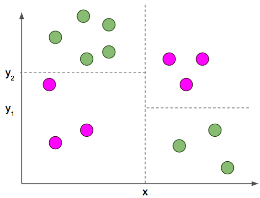
\includegraphics[width=\linewidth]{DecisionTree.png}
  \caption{Decision Tree}
  \label{fig:dt}
\end{figure}

Given training vectors \textit{$x_{i}\epsilon$ $R^{n}$, i=1,..., l} and a label  vector \textit{y$\epsilon$ $R^{l}$}, a decision tree recursively partitions the space such that the samples with the same labels are grouped together.
Let the data at node \textit{m} be represented by \textit{Q}. For each candidate split \textit{$\theta$ \= (j,$t_{m}$)} consisting of a feature \textit{j} and threshold \textit{$t_{m}$} , partition the data into \textit{$Q_{left}$($\theta$)} and \textit{$Q_{right}$($\theta$)} subsets as,
\[ Q_{left}(\theta) = (x,y)|x_{j}<=t_{m}
\]
\[ Q_{right}(\theta) = Q/Q_{left}(\theta)
\]

The impurity at \textit{m} is computed using an impurity function \textit{H()} , the choice of which depends on the task being solved (classification or regression).
\[ G(Q,\theta) = \frac{n_{left}}{N_{m}}H(Q_{left}(\theta)) + \frac{n_{right}}{N_{m}}H(Q_{right}(\theta))
\]
Select the parameters that minimises the impurity
\[ \theta^{\ast} = arg min_{\theta}G(Q,\theta)
\]
Recurse for subsets \textit{$Q_{left}(\theta^{\ast})$} and \textit{$Q_{right}(\theta^{\ast})$} until the maximum allowable depth is reached, \textit{$N_{m}< min_{samples}$} or \textit{$N_{m}$}=1.
\\

\textbf{Advantages:}\\
\indent $\ast$ Quite Simple to understand, interpret and visualize.\\
\indent $\ast$ Able to handle both numeric as well as categorical data and also multi-output problems.\\\
\indent $\ast$ Uses a white box model. If a given situation is observable in a model, the explanation for the condition is easily explained by boolean logic.\\

\textbf{Disadvantages:}\\
\indent $\ast$ Creation of over-complex trees that do not generalize the data well. Overfitting is a problem in  Decision Tree.\\
\indent $\ast$ Decision trees can be unstable because small variations in the data might result in a completely different tree being generated.\\
\indent $\ast$ For the cases, where some classes dominate creation of biased Decision Tree takes place.\\

%%%%%%%%%%%%%%%%%%%%%%%%%%%%%%%%%%%%%%%%%%%%%%%%%%%%%%%%%%%%%%%%%%%%%%%%%%%%%%%%%%%%%%%

\section{RESULTS AND OBSERVATIONS}

\subsection{Performance Measures}
To evaluate classifier performance in a well effective manner, we need to define the performance measure. A classifier performance measure is a single index that measures the Goodness of the classifiers considered.

We have performed a comparative analysis of our classifiers considering the following performance measures:

\textbf{Accuracy Score:}
This compares the actual outcomes with the predicted outcomes of our classifier for a given input dataset. For best Accuracy Score, the set of labels predicted for a sample must match the corresponding set of labels in y\_true

Precision-Recall is a useful measure of success of prediction when the classes are very imbalanced. In information retrieval, precision is a measure of result relevancy, while recall is a measure of how many truly relevant results are returned.

\textbf{Precision Score:}
This is defined as the number of true positives $(T_{p})$ over the number of true positives plus the number of false positives $(F_{p})$
\[ P = \frac{T_{p}}{T_{p}+F_{p}}\]
The precision is intuitively the ability of the classifier not to label as positive a sample that is negative. 
The best value is 1 and the worst value is 0.

\textbf{Recall Score:}
This is defined as the number of true positives $(T_{p})$ over the number of true positives plus the number of false negatives $(F_{n})$
\[ P = \frac{T_{p}}{T_{p}+F_{n}}\]
The recall is intuitively the ability of the classifier to find all the positive samples. 
The best value is 1 and the worst value is 0.

\textbf{F1 Score:}
This is defined as the interpreted as a weighted average of the precision and recall. It is the harmonic mean of precision and recall.
\[ F1 = 2 \frac{P*R}{P+R}
\]
It is also known as the balanced F-score or F-measure. The relative contribution of precision and recall to the F1 score are equal.

\textbf{Average Precision Score:}
This summarizes a precision-recall curve as the weighted mean of precisions achieved at each threshold, with the increase in recall from the previous threshold used as the weight:
\[ AP = \Sigma_{n}(R_{n}-R_{n-1)P_{n}}\]
where \textit{$P_{n}$} and \textit{$R_{n}$} are the precision and recall at the \textit{$n^{th}$} threshold.

\subsection{Comparative Analysis}
\textbf{Accuracy Score:}
\begin{figure}[h!]
  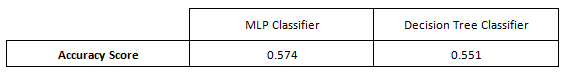
\includegraphics[width=\linewidth]{ModelScore.png}
  \label{fig:scoremodel}
\end{figure}

\textbf{Observation:}
We selected 3 teams: India, Australia and Pakistan randomly and separated the match records of these 3 teams to obtain the performance measure for them separately.
\begin{figure}[h!]
  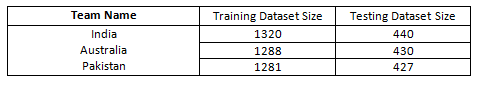
\includegraphics[width=\linewidth]{DatasetTeam.png}
  \label{fig:teamdata}
\end{figure}

\begin{figure}[h!]
  \centering
  \begin{subfigure}[b]{0.4\linewidth}
    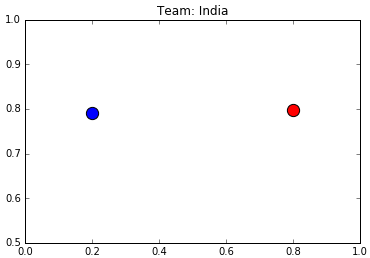
\includegraphics[width=\linewidth]{MLPCLF_India.png}
    \caption{R = 0.797 ,P = 0.791}
  \end{subfigure}
  \begin{subfigure}[b]{0.4\linewidth}
    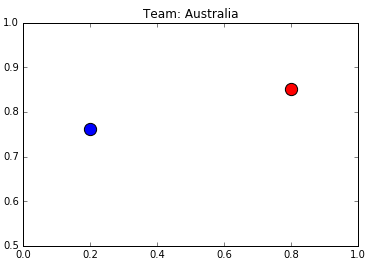
\includegraphics[width=\linewidth]{MLPCLF_Australia.png}
    \caption{R = 0.850 ,P = 0.760}
  \end{subfigure}
  \begin{subfigure}[b]{0.4\linewidth}
    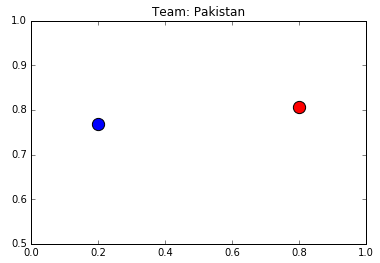
\includegraphics[width=\linewidth]{MLPCLF_Pakistan.png}
    \caption{R = 0.806,P = 0.767}
  \end{subfigure}
  \caption{Recall-Precision Scatter Plot for MLP Classifier.}
  \label{fig:mlpclfPlots}
\end{figure}

\begin{figure}[h!]
  \centering
  \begin{subfigure}[b]{0.4\linewidth}
    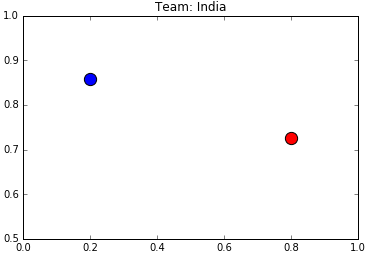
\includegraphics[width=\linewidth]{DTCLF_India.png}
    \caption{R = 0.726,R = 0.859}
  \end{subfigure}
  \begin{subfigure}[b]{0.4\linewidth}
    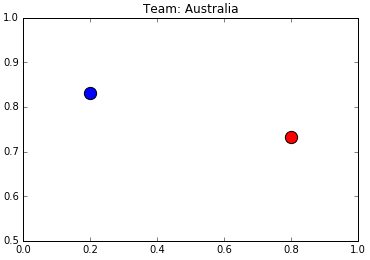
\includegraphics[width=\linewidth]{DTCLF_Australia.png}
    \caption{R = 0.733,P = 0.830}
  \end{subfigure}
  \begin{subfigure}[b]{0.4\linewidth}
    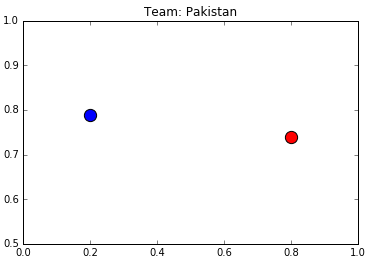
\includegraphics[width=\linewidth]{DTCLF_Pakistan.png}
    \caption{R = 0.739,R = 0.789}
  \end{subfigure}
  \caption{Recall-Precision Scatter Plot for DT Classifier.}
  \label{fig:dtclfPlots}
\end{figure}

\begin{figure}[h!]
  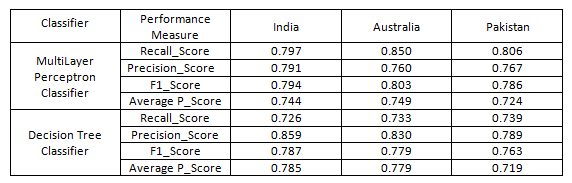
\includegraphics[width=\linewidth]{TeamScore.png}
  \label{fig:results}
\end{figure}

%%%%%%%%%%%%%%%%%%%%%%%%%%%%%%%%%%%%%%%%%%%%%%%%%%%%%%%%%%%%%%%%%%%%%%%%%%%%%%%%%%%%%%%

\section{RELATED WORK}
From our literature survey, we found that very limited machine learning work has been done on game of cricket.  Though cricket shares some attributes with other sports such as baseball, it still remains unique in certain respects and deserves to be analyzed independently.

Most of analyzing studies on cricket so far have been conducted using statistical methods.

Bailey and Clarke conducted a study to predict the outcome in one day international cricket while the game is in progress[5]. WASP(Winning and Score Predictor), 2012 is product of some extensive research of Dr. Scott Brooker and Dr. Seamus Hogan at University of Canterbury in New Zealand. The WASP System is grounded on the theory of Dynamic Programming.

Neeraj Pathak \& Hardik Wadhwa conducted a similar comparative analysis of a match outcomes using the classification models: Support Vector Machines, Random Forests and Naive Bayes[6].Preeti Satao and Team predicted the score of cricket match using Clustering Techniques[7].

Parag Shah, Mitesh Shah[8] and Amal Kaluarachchi, Aparna S. Varde[9] explored the statistical significance for a range of variables that could explain the outcome of an ODI cricket match. In particular, home field advantage, game plan (batting first or fielding first), match type (day or day \& night), past performance of team were the key interests in their investigation.

Madan Gopal Jhanwar and Vikram Pudi embarked on predicting the outcome of a One Day International (ODI) cricket match using a supervised learning approach from a team composition perspective[10]. Their work suggests that the relative team strength between the competing teams forms a distinctive feature for predicting the winner. Swetha and Saravanan.KN analysed the  factors that cricket game depends on and decides Winning[1]. 

%%%%%%%%%%%%%%%%%%%%%%%%%%%%%%%%%%%%%%%%%%%%%%%%%%%%%%%%%%%%%%%%%%%%%%%%%%%%%%%%%%%%%%%

\section{CONCLUSION}

In our study, we performed a comparative analysis of the predictions generated by 2 different supervised classification models for the same input dataset. We have been able to predict the match outcome using the features from the dataset. 

The main contributions of our work are:
\begin{description}
  \item$\bullet$ Comparative analysis of performance measure of two different supervised learning techniques. 
  \item$\bullet$ Analysis of factors that affect the outcome of the game.
  \item$\bullet$ Development of the Prediction tool that can be used to predict the chances of winning, using input attributes.
\end{description}

As future work, we plan to expand this analysis more from the team composition perspective. Also the relevancy of considering 1980s match data equivalent to the 2017s match data also need to be analysed and worked upon. It is also possible to apply the machine learning techniques we used in our study for predicting the outcomes of other games such as hockey and soccer.
%%%%%%%%%%%%%%%%%%%%%%%%%%%%%%%%%%%%%%%%%%%%%%%%%%%%%%%%%%%%%%%%%%%%%%%%%%%%%%%%%%%%%%%

\section{ACKNOWLEDGMENT}

This research was supported by the Department of Computer Science and Engineering, NIT Hamirpur, India. 

We thank our colleagues who provided insight and expertise that greatly assisted the research. 

We are also immensely grateful to them for their comments on an earlier version of the manuscript, although any errors are our own and should not tarnish the reputations of these esteemed persons.

%%%%%%%%%%%%%%%%%%%%%%%%%%%%%%%%%%%%%%%%%%%%%%%%%%%%%%%%%%%%%%%%%%%%%%%%%%%%%%%%


\begin{thebibliography}{99}

\bibitem{c1} Swetha and Saravanan KN, "Analysis on Attributes Deciding Cricket Winning", International Research Journal of Engineering and Technology (IRJET), p-ISSN: 2395-0072, Volume: 04 Issue: 03 — March-2017
\bibitem{c2} Mehvish Khan and Riddhi Shah. "Role of External Factors on Outcome of a One Day International Cricket (ODI) Match and Predictive Analysis", International Journal of Advanced Research in Computer and Communication Engineering Vol. 4, Issue 6, June 2015.
\bibitem{c3} ESPN Cricinfo, http://www.stats.espncricinfo.com
\bibitem{c4} Scikit learn, http://scikit-learn.org/stable/index.html
\bibitem{c5} Bailey and Clarke, Journal of Sports Science and Medicine, 2006, Vol. 5, pp. 480487.
\bibitem{c6} Neeraj Pathak and Hardik Wadhwa,"Applications of modern classification techniques to predict the outcome of ODI Cricket". 2016 International Conference on Computational Science.
\bibitem{c7} "CRICKET SCORE PREDICTION SYSTEM (CSPS) USING CLUSTERING ALGORITHM", Preeti Satao, Ashutosh Tripathi, Jayesh Vankar, Bhavesh Vaje, Vinay Varekar.  International Journal Of Current Engineering and Scientific Research (IJCESR), 23940697, Volume-3, Issue-4, 2016.
\bibitem{c8} Parag Shah and Mitesh Shah, "Predicting ODI Cricket Result". Journal of Tourism, Hospitality and Sports, 2312-5179, Vol.5, 2015.
\bibitem{c9} Kaluarachchi, Amal, and S. Varde Aparna. ”CricAI: A classification based tool to predict the outcome in ODI cricket.” 2010 Fifth International Conference on Information and Automation for Sustainability. IEEE, 2010.
\bibitem{c10}  Madan Gopal Jhanwar and Vikram Pudi, "Predicting the Outcome of ODI Cricket Matches: A Team Composition Based Approach", European Conference on Machine Learning and Principles and Practice of Knowledge Discovery in Databases, Report No: IIIT/TR/2016/-1, Conference Center, Riva del Garda.

\end{thebibliography}

\end{document}
